\documentclass[10pt]{beamer}

\usepackage[utf8]{inputenc}
\usetheme{Berkeley}
\usecolortheme{spruce}

% for degree symbol
\usepackage{textcomp}
\usepackage{tikz}

\setbeamerfont{section in sidebar}{size=\fontsize{5pt}{5pt}}
\setbeamerfont{subsection in sidebar}{size=\fontsize{4pt}{4pt}}

\graphicspath{{./images/}}

%Information to be included in the title page:
\title{Title}
\subtitle{Subtitle}
\author{Matteo Savatteri}
\institute{Università degli Studi di Milano}
\date{\today}

\begin{document}

\frame{\titlepage}

\section*{Outline}
\begin{frame}
\frametitle{Table of Contents}
\tableofcontents
\end{frame}

\section{Introduction}
\subsection{CMB Radiation and B-Modes}

\begin{frame}
\frametitle{CMB Radiation}

\begin{itemize}
\item $\sim$380000 after Big Bang $\rightarrow$ 3000 K $\rightarrow$ recombination $\rightarrow$
      black body radiation \pause
\item Universe expansion $\rightarrow$ 2.7255 K \pause
\item $T$ anisotropies $\rightarrow$ signature primordial perturbations \pause
\end{itemize}

\vspace{15pt}

Thomson Scattering $T$ anisotropies $\rightarrow$ CMB Polarization: \pause
\begin{itemize}
\item E-modes $\rightarrow$ even parity \pause
\item B-modes $\rightarrow$ odd parity
\end{itemize} 

\end{frame}

\begin{frame}
\frametitle{PGW B-modes}

\begin{itemize}
\pause
\item high $l$ $\rightarrow$ gravitational lensing E-modes\pause
\item low $l$ $\rightarrow$ \alert{primordial gravitational waves}: \pause
\begin{itemize}
\item $\frac{\Delta T}{T} \leq 10^{-6}$ \pause
\item Smoking gun inflactionary paradigm
\end{itemize}
\end{itemize}

\end{frame}

\subsection{LSPE/Strip}

\begin{frame}
\frametitle{LSPE/Strip}

\centering
\includegraphics<1>[height=0.75\textheight]{strip-telescope}
\includegraphics<2>[height=0.75\textheight]{strip-focal-plane}

\end{frame}

\section{Atmospheric Emission Model}
\subsection{Equation of Atmospheric Radiative Transfer}

\begin{frame}
\frametitle{Atmospheric Radiative Transfer}

\begin{block}{Radiative Transfer Equation}
\begin{equation}
\frac{dI_\nu}{ds} = -\alpha I_\nu + j_\nu
\end{equation}
\end{block}

\end{frame}

\subsection{Atmospheric Brightness Temperature}

\begin{frame}
\frametitle{Atmospheric Brightness Temperature}

\begin{block}{Atmospheric Brightness Temperature}
\begin{equation}
T_{atm}^A = T_{sky} - T_{CMB}e^{-\tau}
\end{equation}
\end{block}

\end{frame}

\section{Atmospheric Statistical Picture}

\subsection{ERA5 Atmospheric Reanalisys}

\begin{frame}
\frametitle{ERA5 Atmospheric Reanalisys}

\begin{itemize}
\item Earth covered \pause
\item $\sim$40 years of data (1980-2020) \pause
\item Spatial resolution $\rightarrow$ 0.25\textdegree ($\sim$30 Km) \pause
\item Temporal resolution $\rightarrow$ 1 hour \pause

\begin{tikzpicture}[remember picture,overlay]
\node at (4,1) {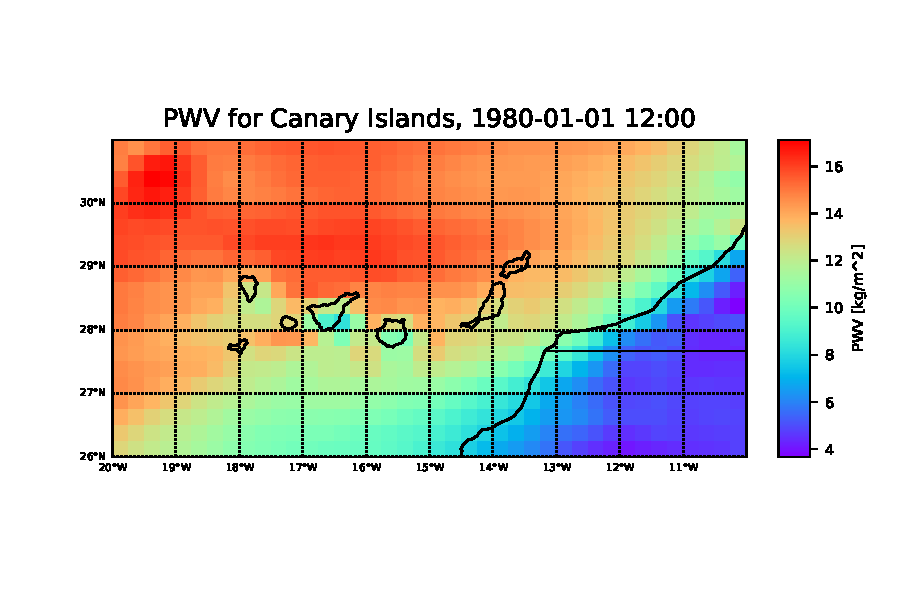
\includegraphics[width=1.2\textwidth]{PWV_Canary_Islands_1980-01-01_12-00}};
\end{tikzpicture}

\end{itemize}

\end{frame}

\subsection{CDFs .fits File}

\begin{frame}
\frametitle{CDFs .fits File}

\includegraphics<1>[height=0.75\textheight]{PWV_Monthly_CDFs/PWV_Monthly_CDFs_Hour_0}
\includegraphics<2>[height=0.75\textheight]{PWV_Monthly_CDFs/PWV_Monthly_CDFs_Hour_5}
\includegraphics<3>[height=0.75\textheight]{PWV_Monthly_CDFs/PWV_Monthly_CDFs_Hour_11}
\includegraphics<4>[height=0.75\textheight]{PWV_Monthly_CDFs/PWV_Monthly_CDFs_Hour_17}

\end{frame}

\section{Comparison with Measurements}
\subsection{Raw Simulation-QUIJOTE Data Comparison}

\begin{frame}
\frametitle{Comparison with QUIJOTE Data}

\includegraphics<1>[height=0.75\textheight]{QUIJOTE-Sim_raw/QUIJOTE_Sim_Comparison_no_cal_11GHz}
\includegraphics<2>[height=0.75\textheight]{QUIJOTE-Sim_raw/QUIJOTE_Sim_Comparison_no_cal_13GHz}
\includegraphics<3>[height=0.75\textheight]{QUIJOTE-Sim_raw/QUIJOTE_Sim_Comparison_no_cal_17GHz}
\includegraphics<4>[height=0.75\textheight]{QUIJOTE-Sim_raw/QUIJOTE_Sim_Comparison_no_cal_19GHz}

\end{frame}


\subsection{Calibrated Simulation-QUIJOTE Data Comparison}

\begin{frame}
\frametitle{Comparison with QUIJOTE Data: Calibrated Simulations}

\includegraphics<1>[height=0.75\textheight]{QUIJOTE-Sim_cal/QUIJOTE_Sim_Comparison_11GHz}
\includegraphics<2>[height=0.75\textheight]{QUIJOTE-Sim_cal/QUIJOTE_Sim_Comparison_13GHz}
\includegraphics<3>[height=0.75\textheight]{QUIJOTE-Sim_cal/QUIJOTE_Sim_Comparison_17GHz}
\includegraphics<4>[height=0.75\textheight]{QUIJOTE-Sim_cal/QUIJOTE_Sim_Comparison_19GHz}

\end{frame}

\section{Bandshape Integration}

\section{Conclusion}
\begin{frame}
\frametitle{Title}
\end{frame}


\end{document}
